\documentclass[conference,a4paper]{IEEEtran}
\usepackage[T1]{fontenc}
\usepackage[utf8]{inputenc}
\usepackage{amsmath,amssymb}
\usepackage{graphicx,booktabs,array,balance}
\usepackage{tikz}
\usetikzlibrary{positioning,arrows.meta}
\usepackage[hidelinks]{hyperref}
\graphicspath{{figures/}}
\newcommand{\TAddSDB}{55.26}
\newcommand{\ToneAddSDB}{2.23}
\newcommand{\TmaxAddSDB}{114.54}
\newcommand{\TAddDDB}{56.17}
\newcommand{\ToneAddDDB}{2.22}
\newcommand{\TmaxAddDDB}{114.48}
\newcommand{\TSLSDB}{59.01}
\newcommand{\ToneSLSDB}{2.46}
\newcommand{\TmaxSLSDB}{123.90}
\newcommand{\TSLDDB}{60.23}
\newcommand{\ToneSLDDB}{2.46}
\newcommand{\TmaxSLDDB}{129.16}
\newcommand{\TZDB}{63.03}
\newcommand{\ToneZDB}{2.37}
\newcommand{\TmaxZDB}{130.83}
\newcommand{\TAddSC}{54.94}
\newcommand{\ToneAddSC}{1.80}
\newcommand{\TmaxAddSC}{114.93}
\newcommand{\TAddDC}{55.52}
\newcommand{\ToneAddDC}{1.77}
\newcommand{\TmaxAddDC}{109.46}
\newcommand{\TSLSC}{58.58}
\newcommand{\ToneSLSC}{1.82}
\newcommand{\TmaxSLSC}{122.45}
\newcommand{\TSLDC}{60.30}
\newcommand{\ToneSLDC}{1.86}
\newcommand{\TmaxSLDC}{122.70}
\newcommand{\TZC}{62.79}
\newcommand{\ToneZC}{1.89}
\newcommand{\TmaxZC}{131.15}
\newcommand{\DynAddDB}{1.7}
\newcommand{\DynSLDB}{2.1}
\newcommand{\SLvsAddSDB}{6.8}
\newcommand{\SLvsAddDDB}{7.2}
\newcommand{\ZvsSLDDB}{4.7}
\newcommand{\DynAddC}{1.1}
\newcommand{\DynSLC}{2.9}
\newcommand{\SLvsAddSC}{6.6}
\newcommand{\SLvsAddDC}{8.6}
\newcommand{\ZvsSLDC}{4.1}
\newcommand{\CacheSaveS}{0.7}
\newcommand{\CacheSaveD}{-0.1}
\newcommand{\CacheSaveAddS}{0.6}
\newcommand{\CacheSaveOneS}{26}
\newcommand{\CacheSaveOneAddS}{19}
\newcommand{\AucAddS}{0.791}
\newcommand{\RecAddS}{20.7}
\newcommand{\BdAddS}{0.51}
\newcommand{\FoneAddS}{0.335}
\newcommand{\EpAddS}{25.3}
\newcommand{\ExpAddS}{26.0}
\newcommand{\HiAddS}{17.7}
\newcommand{\PrRecAddS}{0.0}
\newcommand{\PrBdAddS}{0.00}
\newcommand{\UsAddS}{5}
\newcommand{\RCredAddS}{100.0}
\newcommand{\RCompAddS}{0.4}
\newcommand{\RLatAddS}{0.0}
\newcommand{\RSlowAddS}{0.1}
\newcommand{\AucAddD}{0.800}
\newcommand{\RecAddD}{20.8}
\newcommand{\BdAddD}{0.59}
\newcommand{\FoneAddD}{0.336}
\newcommand{\EpAddD}{27.7}
\newcommand{\ExpAddD}{25.4}
\newcommand{\HiAddD}{17.6}
\newcommand{\PrRecAddD}{0.0}
\newcommand{\PrBdAddD}{0.00}
\newcommand{\UsAddD}{6}
\newcommand{\RCredAddD}{100.0}
\newcommand{\RCompAddD}{0.7}
\newcommand{\RLatAddD}{0.1}
\newcommand{\RSlowAddD}{0.2}
\newcommand{\AucSLS}{0.753}
\newcommand{\RecSLS}{20.5}
\newcommand{\BdSLS}{0.66}
\newcommand{\FoneSLS}{0.331}
\newcommand{\EpSLS}{25.0}
\newcommand{\ExpSLS}{26.1}
\newcommand{\HiSLS}{17.7}
\newcommand{\PrRecSLS}{0.0}
\newcommand{\PrBdSLS}{0.00}
\newcommand{\UsSLS}{28}
\newcommand{\RCredSLS}{100.0}
\newcommand{\RCompSLS}{0.0}
\newcommand{\RLatSLS}{0.0}
\newcommand{\RSlowSLS}{0.0}
\newcommand{\AucSLD}{0.748}
\newcommand{\RecSLD}{14.6}
\newcommand{\BdSLD}{0.70}
\newcommand{\FoneSLD}{0.247}
\newcommand{\EpSLD}{26.1}
\newcommand{\ExpSLD}{25.9}
\newcommand{\HiSLD}{17.7}
\newcommand{\PrRecSLD}{0.5}
\newcommand{\PrBdSLD}{0.00}
\newcommand{\UsSLD}{36}
\newcommand{\RCredSLD}{70.8}
\newcommand{\RCompSLD}{0.3}
\newcommand{\RLatSLD}{0.1}
\newcommand{\RSlowSLD}{0.0}
\newcommand{\AucCV}{0.819}
\newcommand{\RecCV}{16.7}
\newcommand{\BdCV}{0.72}
\newcommand{\FoneCV}{0.278}
\newcommand{\EpCV}{37.2}
\newcommand{\ExpCV}{24.2}
\newcommand{\HiCV}{17.5}
\newcommand{\PrRecCV}{5.5}
\newcommand{\PrBdCV}{0.05}
\newcommand{\UsCV}{40}
\newcommand{\RCredCV}{72.2}
\newcommand{\RCompCV}{3.4}
\newcommand{\RLatCV}{3.0}
\newcommand{\RSlowCV}{0.2}
\newcommand{\AucMS}{0.852}
\newcommand{\RecMS}{31.9}
\newcommand{\BdMS}{0.72}
\newcommand{\FoneMS}{0.471}
\newcommand{\EpMS}{73.2}
\newcommand{\ExpMS}{13.7}
\newcommand{\HiMS}{13.4}
\newcommand{\PrRecMS}{8.1}
\newcommand{\PrBdMS}{0.00}
\newcommand{\UsMS}{42}
\newcommand{\RCredMS}{91.0}
\newcommand{\RCompMS}{13.0}
\newcommand{\RLatMS}{35.9}
\newcommand{\RSlowMS}{2.8}
\newcommand{\AucLP}{0.765}
\newcommand{\RecLP}{22.6}
\newcommand{\BdLP}{0.71}
\newcommand{\FoneLP}{0.358}
\newcommand{\EpLP}{68.9}
\newcommand{\ExpLP}{12.6}
\newcommand{\HiLP}{15.0}
\newcommand{\PrRecLP}{6.2}
\newcommand{\PrBdLP}{0.01}
\newcommand{\UsLP}{40}
\newcommand{\RCredLP}{70.9}
\newcommand{\RCompLP}{12.2}
\newcommand{\RLatLP}{17.1}
\newcommand{\RSlowLP}{0.0}
\newcommand{\AucCVMS}{0.891}
\newcommand{\RecCVMS}{33.6}
\newcommand{\BdCVMS}{0.66}
\newcommand{\FoneCVMS}{0.490}
\newcommand{\EpCVMS}{77.1}
\newcommand{\ExpCVMS}{13.3}
\newcommand{\HiCVMS}{12.8}
\newcommand{\PrRecCVMS}{13.0}
\newcommand{\PrBdCVMS}{0.04}
\newcommand{\UsCVMS}{45}
\newcommand{\RCredCVMS}{85.9}
\newcommand{\RCompCVMS}{18.6}
\newcommand{\RLatCVMS}{38.3}
\newcommand{\RSlowCVMS}{4.0}
\newcommand{\AucZ}{0.888}
\newcommand{\RecZ}{34.0}
\newcommand{\BdZ}{0.74}
\newcommand{\FoneZ}{0.493}
\newcommand{\EpZ}{77.0}
\newcommand{\ExpZ}{11.1}
\newcommand{\HiZ}{12.6}
\newcommand{\PrRecZ}{15.6}
\newcommand{\PrBdZ}{0.05}
\newcommand{\UsZ}{46}
\newcommand{\RCredZ}{83.4}
\newcommand{\RCompZ}{23.3}
\newcommand{\RLatZ}{38.3}
\newcommand{\RSlowZ}{1.0}
\newcommand{\DAuc}{0.140}
\newcommand{\DAucLo}{0.126}
\newcommand{\DAucHi}{0.154}
\newcommand{\DRec}{19.4}
\newcommand{\DRecLo}{18.7}
\newcommand{\DRecHi}{20.0}
\newcommand{\DFone}{0.246}
\newcommand{\DFoneLo}{0.238}
\newcommand{\DFoneHi}{0.254}
\newcommand{\DEp}{50.9}
\newcommand{\DEpLo}{50.0}
\newcommand{\DEpHi}{51.8}
\newcommand{\DExp}{-14.8}
\newcommand{\DExpLo}{-15.6}
\newcommand{\DExpHi}{-14.0}
\newcommand{\NTest}{163,100}
\newcommand{\NMal}{26,309}
\newcommand{\NBen}{136,791}
\newcommand{\NEp}{800}
\newcommand{\NWarm}{136,245}

\hypersetup{pdftitle={ZT-CMS: Continuous Verification, Micro-Segmentation and Least Privilege for Score-Based Zero Trust Access Control},pdfauthor={Parveen Kumar, Mann, Vishavjeet, Shreevats}}
\title{ZT-CMS: Continuous Verification, Micro-Segmentation and Least Privilege for Score-Based Zero Trust Access Control in Enterprise Networks}
\author{\IEEEauthorblockN{Parveen Kumar (23BCS093), Mann (23BCS078),
Vishavjeet (23BDS069), and Shreevats (23BDS055)}
\IEEEauthorblockA{Indian Institute of Information Technology Dharwad, India}}
\begin{document}
\maketitle
\begin{abstract}
Zero Trust (ZT) enterprise networks grant every resource access request (RAR) only if a trust score exceeds a required threshold. We reproduce the IEEE TrustCom 2023 paper by Bradatsch \emph{et al.}, which defines 29 trust attributes, a dynamic risk-based threshold, and an additive and a Subjective Logic (SL) trust algorithm, and which evaluates decision time only. We rebuild its NIST-style testbed (PEP, PDP, PAP, PIP and a PostgreSQL attribute store over mutual TLS) and repeat its experiment from 1 to 128 concurrent requests. Our reproduction confirms two of its three relative claims: SL costs within about 7\% of the additive algorithm, and a dynamic risk level adds little time; the cache benefit appears only at low load on our single machine. The base paper leaves decision accuracy as future work. We therefore propose ZT-CMS, which keeps the SL algorithm and adds continuous verification (a running per-user and per-device suspicion score), micro-segmentation risk agents (segment novelty and lateral fan-out), and a least-privilege entitlement agent. On \NTest{} labelled requests from five unseen simulated enterprises with four attack types, at a fixed 1\% benign-denial target, ZT-CMS raises ROC AUC from \AucSLD{} to \AucZ{}, malicious-request recall from \RecSLD\% to \RecZ\%, and attack-episode detection from \EpSLD\% to \EpZ\%, compared with the reproduced SL algorithm; it also outperforms the best additive configuration (episode detection \EpAddD\%). It adds \ZvsSLDC\% decision time when attributes are cached.
\end{abstract}
\begin{IEEEkeywords}
Zero Trust, access control, trust score, Subjective Logic, micro-segmentation, continuous verification, least privilege.
\end{IEEEkeywords}

\section{Introduction and Base Paper}
Perimeter security trusts whatever is inside the network, so a stolen password or an infected laptop can move laterally once inside. Zero Trust Architecture (ZTA) removes this implicit trust: a Policy Enforcement Point (PEP) asks a Policy Decision Point (PDP) to authorise every resource access request (RAR), and the PDP decides from attributes of the user, device and channel~\cite{nist}. Score-based ZT computes a trust score for each RAR and grants access only if the score exceeds a threshold~\cite{nist,gilman}.

\subsection{The IEEE paper we implemented}
Our base paper is \emph{Zero Trust Score-based Network-level Access Control in Enterprise Networks} by L.~Bradatsch, O.~Miroshkin, N.~Trkulja and F.~Kargl, IEEE TrustCom 2023~\cite{base}. It contributes (i) 29 trust attributes for three entities (user, device and communication channel) with a model for quantifying their weights, (ii) a dynamic \emph{risk level} computed from 9 risk attributes and used as the threshold, and (iii) an SL trust algorithm compared with a lightweight additive one. Its evaluation measures \emph{decision time only}. With 64 concurrent requests, the reported times are 296\,ms (additive) and 294\,ms (SL) when the Policy Information Point (PIP) queries its database, a 7\% increase for a dynamic risk level (317 and 316\,ms), and 126\,ms (static) or 133\,ms (dynamic) when the PIP serves attributes from a cache. The authors list the accuracy of access decisions (false positives and negatives) as future work~\cite{base}.

\subsection{Problem and contributions}
The base algorithms judge each RAR in isolation. An attacker who keeps every single request ``normal enough'' is never denied, even when the requests together show compromise or lateral movement. Our project topic covers continuous verification, micro-segmentation and least privilege, and each of these addresses part of this gap. We contribute:
\begin{itemize}
\item a working reproduction of the base paper's algorithms and testbed, and a check of its three performance claims (Sec.~\ref{sec:repro});
\item ZT-CMS, three SL-compatible extensions: \textbf{C}ontinuous verification, \textbf{M}icro-\textbf{S}egmentation, and least-privilege scoping (Sec.~\ref{sec:method});
\item the base paper's missing accuracy evaluation: a labelled enterprise simulator with four attacks and a calibrated comparison of all algorithms, including ablations (Sec.~\ref{sec:acc}).
\end{itemize}

\section{Related Work}\label{sec:related}
\emph{Zero Trust architectures.} NIST SP~800-207 defines the logical components of a ZTA (PEP, PDP with Policy Engine and Policy Administrator, and information sources) and names a trust algorithm that may be score-based or criteria-based~\cite{nist}. Google's BeyondCorp moved access decisions from the network perimeter to per-request checks of user and device state~\cite{beyondcorp}, and Gilman and Barth describe trust scores as the central engineering element of such networks~\cite{gilman}. Surveys find that most ZT publications stay conceptual, and that concrete trust algorithms and their empirical evaluation are a main research gap~\cite{syed,buck}.

\emph{Trust algorithms and continuous authorisation.} Dimitrakos \emph{et al.} add trust-aware continuous authorisation to attribute-based access control, re-evaluating sessions as context changes~\cite{dimitrakos}. Bradatsch \emph{et al.}, our base paper, give the most complete published network-level score-based design: an explicit attribute catalogue, a dynamic risk threshold and two trust algorithms, with open-source code~\cite{base,repo}. Subjective Logic~\cite{josang} and its multi-source fusion operators~\cite{fusion} provide the uncertainty-aware reasoning that its second algorithm uses.

\emph{Positioning.} Prior score-based designs, including the base paper, evaluate a single request at a time and report performance rather than decision accuracy. Our work keeps the base design intact, measures its accuracy for the first time on labelled traffic, and adds memory across requests (continuous verification), segment awareness (micro-segmentation) and role scoping (least privilege). For accumulating weak evidence we borrow the classic CUSUM idea from statistical change detection~\cite{page}.

\section{Base Paper Method}\label{sec:base}
\subsection{Architecture and attributes}
Following NIST SP~800-207~\cite{nist}, the PEP sends a decision request to the PDP. Its Policy Engine fetches a score-based policy from the Policy Administration Point (PAP) and attribute values from the PIP. The trust algorithm then compares the trust score with a threshold. The 29 trust attributes are split by entity: 10 for the user (e.g.\ authentication factors, access time, service usage), 16 for the device (e.g.\ managed state, patch level, fingerprint, location, vulnerability scan), and 3 for the channel (authentication, confidentiality, integrity). The 9 risk attributes describe the request (protocol, action, data sensitivity), the target system (patch level, state, threat level) and the network (state, threat level)~\cite{base}.

\subsection{Additive algorithm}
Every trust attribute that is satisfied adds its expert weight to a total trust score. The risk attributes are added up in the same way to form the risk level, which acts as the threshold. Access is granted only if the trust score is higher than the risk level. The algorithm is fast and easy to explain, but one very trusted entity, such as a well-managed device, can make up for an untrusted user.

\subsection{Subjective Logic algorithm}
Subjective Logic (SL)~\cite{josang} lets each attribute express not only how good or bad it looks but also how \emph{certain} that evidence is. Each trust attribute is evaluated by an agent that forms an opinion made of belief, disbelief and uncertainty. The opinions about one entity are merged by weighted belief fusion, in which more certain agents count more~\cite{fusion}. Risk opinions are merged by cumulative belief fusion, so that independent risks add up. Each merged opinion is turned into a single score between 0 and 1. Access is granted only if the user score, the device score and the channel score are \emph{each} higher than the risk score. Checking the entities separately prevents a trusted device from compensating an untrusted user. With a \emph{static} risk level the threshold is a constant; with a \emph{dynamic} one it is computed for each request.

\section{Proposed ZT-CMS Extensions}\label{sec:method}
ZT-CMS keeps the base SL algorithm with a dynamic risk level. It changes only (a) the entity trust scores and (b) the set of risk agents (Fig.~\ref{fig:arch}). Each component can be switched off for ablation.

\begin{figure}[t]\centering
\resizebox{\columnwidth}{!}{%
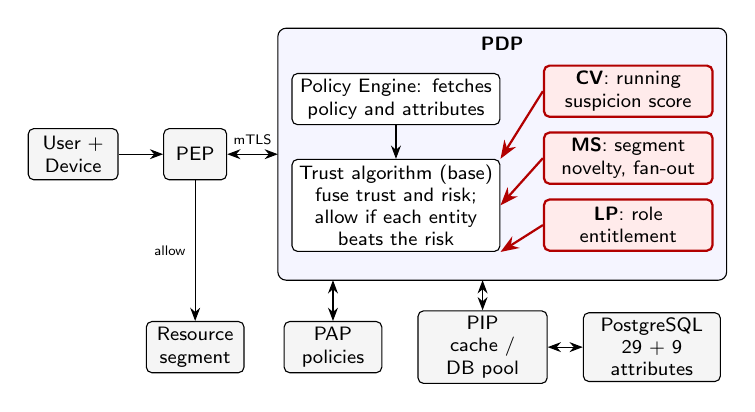
\begin{tikzpicture}[font=\sffamily\scriptsize, >=Stealth,
  box/.style={draw, rounded corners=2pt, align=center, minimum height=6.5mm, fill=gray!8, inner sep=2pt},
  ours/.style={draw=red!70!black, thick, rounded corners=2pt, align=center, fill=red!8, text width=20mm, minimum height=6.5mm, inner sep=2pt}]
\node[box, text width=10mm] (user) at (0,0) {User +\\Device};
\node[box, minimum width=8mm] (pep) at (1.55,0) {PEP};
\draw[rounded corners=3pt, fill=blue!4] (2.6,-1.6) rectangle (8.3,1.6);
\node at (5.45,1.4) {\textbf{PDP}};
\node[box, fill=white, text width=25mm] (pe) at (4.1,0.7) {Policy Engine: fetches\\policy and attributes};
\node[box, fill=white, text width=25mm] (ta) at (4.1,-0.65) {Trust algorithm (base)\\fuse trust and risk;\\allow if each entity\\beats the risk};
\node[ours] (cv) at (7.05,0.8) {\textbf{CV}: running\\suspicion score};
\node[ours] (ms) at (7.05,-0.05) {\textbf{MS}: segment\\novelty, fan-out};
\node[ours] (lp) at (7.05,-0.9) {\textbf{LP}: role\\entitlement};
\node[box, text width=11mm] (pap) at (3.3,-2.45) {PAP\\policies};
\node[box, text width=15mm] (pip) at (5.2,-2.45) {PIP\\cache / DB pool};
\node[box, text width=16mm] (db) at (7.35,-2.45) {PostgreSQL\\29 + 9 attributes};
\node[box, text width=11mm] (res) at (1.55,-2.45) {Resource\\segment};
\draw[->] (user) -- (pep);
\draw[<->] (pep.east) -- node[above, font=\sffamily\tiny]{mTLS} (2.6,0);
\draw[->] (pe) -- (ta);
\draw[->, red!70!black, thick] (cv.west) -- (ta.north east);
\draw[->, red!70!black, thick] (ms.west) -- (ta.east);
\draw[->, red!70!black, thick] (lp.west) -- (ta.south east);
\draw[<->] (pap.north) -- (3.3,-1.6);
\draw[<->] (pip.north) -- (5.2,-1.6);
\draw[<->] (pip) -- (db);
\draw[->] (pep.south) -- node[left, font=\sffamily\tiny]{allow} (res.north);
\end{tikzpicture}}
\caption{Base architecture of~\cite{base} (grey/blue, NIST SP 800-207) with the three ZT-CMS additions (red). CV lowers user and device trust; MS and LP add new risk agents.}\label{fig:arch}
\end{figure}

\subsection{Continuous verification (CV)}
In the base paper a weak signal never accumulates: thirty slightly suspicious requests are judged like one. ZT-CMS therefore keeps a running suspicion score for every user and every device, in the spirit of the cumulative-sum (CUSUM) change detector~\cite{page}. Each request adds the amount by which that entity's SL disbelief exceeds the entity's \emph{own} normal level, learned during a benign warm-up week. The score fades over time with a two-hour time constant, and the entity's trust is lowered in proportion to it. Comparing each entity with its own history, rather than with a global average, avoids penalising users whose personal laptops always look slightly worse. A device never seen before first learns its own normal level from its first ten requests, while the base per-request check still applies. Each request can add only a small amount, so large one-off changes are left to the base check and the running score targets small persistent shifts. Because old evidence fades, a single anomaly does not lock a user out.

\subsection{Micro-segmentation (MS)}
Resources are grouped into micro-segments with sensitivity tiers. Two new risk agents join the risk opinion. A \emph{segment-novelty} agent reports strong evidence of risk when a user requests a segment outside the set they normally used during warm-up. A \emph{lateral fan-out} agent reports evidence that grows with the number of distinct segments the user has touched in the last hour beyond that user's usual maximum. Lateral movement therefore raises the required trust even when every credential and device attribute looks normal.

\subsection{Least privilege (LP)}
A role-entitlement agent reports full evidence of risk when the requested segment is outside the user's role. The request is not hard-blocked; instead, out-of-role access must be backed by higher trust, so help-desk-style exceptions remain possible. The decision rule is otherwise unchanged: every entity's trust, after the CV adjustment, must exceed the extended risk score. Table~\ref{tab:comp} summarises the three components.
\begin{table}[t]\caption{ZT-CMS components and the Zero Trust principle each enforces}\label{tab:comp}
\centering\small\setlength{\tabcolsep}{3pt}
\begin{tabular}{p{.17\columnwidth}p{.37\columnwidth}p{.38\columnwidth}}\toprule
Part & Signal it uses & Effect on the decision\\\midrule
CV & Repeated small anomalies of a user or device, against its own history & Lowers that entity's trust; fades within hours\\
MS & New segment for this user; many segments in one hour & Adds risk, so lateral movement needs more trust\\
LP & Segment outside the user's role & Adds risk; out-of-role access needs higher trust, no hard block\\\bottomrule
\end{tabular}\end{table}


\begin{figure*}[t]\centering
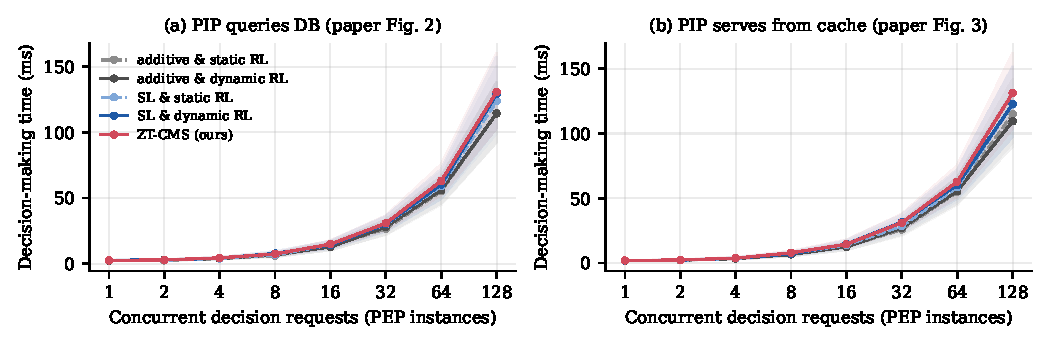
\includegraphics[width=.92\textwidth]{decision_time.pdf}
\caption{Reproduction of the base paper's decision-time experiment. Lines show the median and bands the inter-quartile range over all requests and three repetitions. ZT-CMS (red) is our extension, measured on the same path.}\label{fig:time}
\end{figure*}

\section{Implementation and Experimental Setup}\label{sec:setup}
\subsection{Reproduction testbed}
We implement PEP, PDP, PAP and PIP as separate Python 3.13 processes communicating over REST with mutual TLS~1.3, as in the base paper's Fig.~1. The PIP reads attributes from a dedicated PostgreSQL~16 database in one SQL batch per request, through a bounded pool of 16 connections, as Go's \texttt{database/sql} in the authors' implementation~\cite{repo} also pools connections. The dynamic risk level adds the resource's risk attributes to that batch. As in the paper, the database holds dummy values for all 29 trust and 9 risk attributes. We repeat the base protocol: 1 to 128 parallel PEP instances, with the PIP either querying the database (paper Fig.~2) or serving all attributes from its cache (paper Fig.~3). Decision time is measured at the PEP from sending the decision request to receiving the decision. We use 50 requests per instance and 3 repetitions (paper: 1000 and 10). Within each repetition and concurrency level, the five configurations are measured back to back in alternating order, so slow drift such as thermal throttling affects all of them equally. Everything runs on one laptop: an AMD Ryzen~7 5800H with 16 logical CPUs running Windows~11. The paper used four 32-core Xeon servers connected by 100\,GbE.

\subsection{Labelled enterprise simulator}
Each simulated enterprise has 200 users in six roles, 10 micro-segments in four sensitivity tiers (e.g.\ intranet, GitLab, HR portal, customer DB, production Kubernetes, AD admin) and 14 days of traffic. Each RAR carries all 29 trust and 9 risk attributes. Benign traffic includes realistic noise: personal unmanaged devices (20\% of users), travel, new-device enrolment, patch lag, password typos, late work, request bursts, network-threat days and occasional out-of-role access. Days 0--6 are benign warm-up, used only to learn ZT-CMS norms. On days 7--13, 40 episodes of each attack in Table~\ref{tab:attacks} are mixed with benign traffic.

\begin{table}[t]\caption{Attack episodes injected on days 7--13}\label{tab:attacks}
\centering\small\setlength{\tabcolsep}{3pt}
\begin{tabular}{p{.27\columnwidth}p{.67\columnwidth}}\toprule
Attack & What changes\\\midrule
Credential theft & Stolen password (50\% also pass MFA) used from an unknown, unmanaged device; 15--40 RARs, half to tier 2 or higher.\\
Compromised device & Malware on the victim's managed laptop: slightly worse health and scan status, occasional TLS downgrade; 30--60 slow RARs.\\
Lateral movement & Valid user and device sweep many segments, including out-of-role ones; 20--40 RARs.\\
Slow exfiltration & Insider repeatedly reads one entitled but unusual high-tier segment, often after hours, over 3 days.\\\bottomrule
\end{tabular}\end{table}

\subsection{Protocol and metrics}
All algorithms use one shared expert weight table and see identical requests. We report two operating points. The \emph{paper rule} grants access exactly when trust exceeds risk, as in the base paper. Because expert weights set the scale arbitrarily, we also use a \emph{calibrated} point: each algorithm's threshold is fixed on a separate calibration enterprise (seed 101) so that 1\% of benign RARs are denied. That threshold is then applied unchanged to five unseen test enterprises (seeds 201--205: \NTest{} test RARs, of which \NMal{} are malicious, in \NEp{} episodes). ZT-CMS hyperparameters were chosen on a separate development enterprise (seed 301). We report ROC AUC (threshold-free), recall, benign-denial rate, F1, episode detection (at least one denial), and exposure (malicious RARs allowed before the first denial). Differences between methods are paired by enterprise and reported with 95\% confidence intervals.

\begin{table*}[t]\caption{Decision accuracy on five unseen test enterprises (mean $\pm$ s.d.). Calibrated: threshold fixed on a separate enterprise to deny 1\% of benign requests.}\label{tab:acc}\centering\small\setlength{\tabcolsep}{4pt}
\begin{tabular}{lcccccccc}\toprule
 & \multicolumn{2}{c}{Paper rule (trust exceeds risk)} & \multicolumn{6}{c}{Calibrated (1\% benign denial target)}\\\cmidrule(lr){2-3}\cmidrule(lr){4-9}
Algorithm & Recall & Benign deny & AUC & Recall & Benign deny & F1 & Episodes det. & Exposure\\\midrule
Additive-static & 0.000 & 0.000 & 0.791$\pm$0.010 & 0.207 & 0.005 & 0.335 & 0.253 & 26.0\\
Additive-dynamic & 0.000 & 0.000 & 0.800$\pm$0.016 & 0.208 & 0.006 & 0.336 & 0.277 & 25.4\\
\midrule
SL-static & 0.000 & 0.000 & 0.753$\pm$0.012 & 0.205 & 0.007 & 0.331 & 0.250 & 26.1\\
SL-dynamic & 0.005 & 0.000 & 0.748$\pm$0.018 & 0.146 & 0.007 & 0.247 & 0.261 & 25.9\\
\midrule
SL-dyn + CV & 0.055 & 0.000 & 0.819$\pm$0.019 & 0.167 & 0.007 & 0.278 & 0.372 & 24.2\\
SL-dyn + MS & 0.081 & 0.000 & 0.852$\pm$0.008 & 0.319 & 0.007 & 0.471 & 0.733 & 13.7\\
SL-dyn + LP & 0.062 & 0.000 & 0.765$\pm$0.014 & 0.226 & 0.007 & 0.358 & 0.689 & 12.6\\
SL-dyn + CV+MS & 0.130 & 0.000 & 0.891$\pm$0.009 & 0.336 & 0.007 & 0.490 & 0.771 & 13.3\\
\midrule
\textbf{ZT-CMS (ours)} & 0.156 & 0.000 & 0.888$\pm$0.009 & 0.340 & 0.007 & 0.493 & 0.770 & 11.1\\
\bottomrule\end{tabular}\end{table*}


\section{Results}
\subsection{Reproduction of the base paper's performance}\label{sec:repro}
\begin{table}[t]\caption{Decision time at 64 concurrent requests: paper vs.\ our reproduction}\label{tab:repro}\centering\small\setlength{\tabcolsep}{3.5pt}
\begin{tabular}{llrr}\toprule
PIP & Configuration & Paper (ms) & Ours (ms)\\\midrule
DB & additive \& static RL & 296 & 55.26\\
DB & SL \& static RL & 294 & 59.01\\
DB & additive \& dynamic RL & 317 & 56.17\\
DB & SL \& dynamic RL & 316 & 60.23\\
DB & ZT-CMS (ours) & -- & 63.03\\
\midrule
Cache & additive \& static RL & 126 & 54.94\\
Cache & SL \& static RL & 126 & 58.58\\
Cache & additive \& dynamic RL & 133 & 55.52\\
Cache & SL \& dynamic RL & 133 & 60.30\\
Cache & ZT-CMS (ours) & -- & 62.79\\
\bottomrule\end{tabular}\end{table}

Table~\ref{tab:repro} and Fig.~\ref{fig:time} compare our decision times with the paper's. Absolute times are not comparable: all components, the database and the load generator share one laptop and loopback links, whereas the paper used four dedicated servers. We therefore check the paper's three \emph{relative} claims at 64 concurrent requests. (i)~\emph{SL costs about the same as additive} (paper: 294 vs.\ 296\,ms). This holds approximately: SL is \SLvsAddSDB\% slower with database access and \SLvsAddSC\% slower with the cache. Pure computation is \UsAddS\,\textmu s (additive) versus \UsSLS\,\textmu s (SL) per decision, the same order as the paper's 10--40\,\textmu s; a likely reason for the small gap is that on a saturated laptop the extra CPU time per decision turns into queueing delay. (ii)~\emph{A dynamic risk level adds little} (paper: 7\%). This holds: \DynAddDB\% for additive and \DynSLDB\% for SL with database access. (iii)~\emph{An attribute cache shortens decisions} (paper: 294 to 126\,ms). This holds only at low load. With a single PEP the cache saves \CacheSaveOneS\% for SL and \CacheSaveOneAddS\% for additive, but at 64 concurrent requests the difference is below 1\%, because the shared CPU, not the database, is then the bottleneck. In all configurations decision time grows with concurrency, as in the paper's figures. Our first timing run measured the configurations one after another and was biased by thermal throttling (Sec.~\ref{sec:disc}); all numbers here come from the interleaved run.



\subsection{Decision accuracy (base paper's future work)}\label{sec:acc}
\emph{Paper rule.} Under the paper's own rule the shared expert weights let almost every RAR through. The additive and SL baselines deny at most \PrRecSLD\% of malicious RARs (Table~\ref{tab:acc}). This shows the weight-calibration problem that the base paper itself raises: without calibration the rule ``grant if trust exceeds risk'' depends entirely on the arbitrary weight scale.

\emph{Calibrated comparison.} At the same 1\% benign-denial target, the reproduced SL algorithm with dynamic risk reaches AUC \AucSLD{}, recall \RecSLD\% and episode detection \EpSLD\%. The strongest base configuration is the additive algorithm with dynamic risk (AUC \AucAddD{}, recall \RecAddD\%, episode detection \EpAddD\%). SL ranks requests worse than additive scoring; a likely reason is that WBF weights each agent by its certainty, so one strong but uncertain warning, such as an unknown device, is diluted by many confident normal attributes. ZT-CMS reaches AUC \AucZ{}, recall \RecZ\%, F1 \FoneZ{} and episode detection \EpZ\%, and it reduces exposure from \ExpSLD{} to \ExpZ{} allowed malicious RARs per episode. Paired over the five unseen enterprises, the AUC gain is \DAuc{} (95\% CI [\DAucLo, \DAucHi]), the recall gain is \DRec{} points ([\DRecLo, \DRecHi]) and the episode-detection gain is \DEp{} points ([\DEpLo, \DEpHi]). ZT-CMS also exceeds the additive baseline on every aggregate metric in Table~\ref{tab:acc}. The realised benign-denial rate on the test enterprises is \BdZ\% for ZT-CMS versus \BdSLD\% for SL, so the gains do not come from denying more legitimate users.



\emph{Per attack} (Fig.~\ref{fig:attacks}). The additive algorithm catches credential theft in a single request (\RCredAddD\%), because an unknown, unmanaged device removes large weights. SL dilutes this signal (\RCredSLD\%), and ZT-CMS recovers part of it (\RCredZ\%) through segment novelty. The extensions matter most for attacks that use valid credentials and devices, which every base configuration misses: lateral-movement recall rises from \RLatSLD\% to \RLatZ\% and compromised-device recall from \RCompSLD\% to \RCompZ\%. Slow exfiltration over three days stays undetected by every method (at most \RSlowCVMS\%), because its evidence fades between days.

\begin{figure}[t]\centering
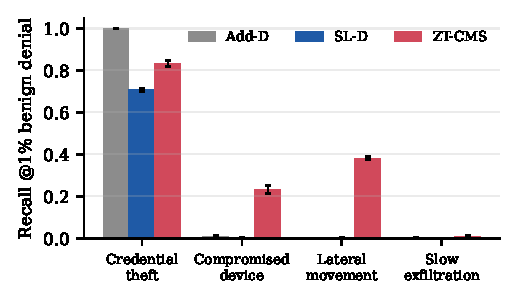
\includegraphics[width=\columnwidth]{attacks.pdf}
\caption{Recall per attack type at the calibrated 1\% benign-denial point.}\label{fig:attacks}
\end{figure}

\emph{Ablation.} Each component improves on the SL baseline by itself (Table~\ref{tab:acc}). MS gives the largest single gain (recall \RecMS\%, episode detection \EpMS\%). LP gives the lowest single-component exposure (\ExpLP). CV mainly improves the threshold-free ranking (AUC \AucSLD{} to \AucCV) but adds little recall at the 1\% point, because benign posture changes such as patch lag or a newly enrolled device also accumulate disbelief. CV and MS together give the best AUC (\AucCVMS). Adding LP leaves AUC and episode detection essentially unchanged (\AucZ, \EpZ\%), but it lowers exposure further (\ExpCVMS{} to \ExpZ) and raises compromised-device recall (\RCompCVMS\% to \RCompZ\%).

\subsection{Cost of the extensions}
ZT-CMS needs \UsZ\,\textmu s of pure computation per decision versus \UsSLD\,\textmu s for SL. On the full mutual-TLS path at 64 concurrent requests, it adds \ZvsSLDC\% decision time with the cache and \ZvsSLDDB\% with database access (Table~\ref{tab:repro}). As in the base paper, the trust calculation itself is a small part of the request path; TLS, network and attribute retrieval dominate.

\section{Discussion and Limitations}\label{sec:disc}
\emph{What the comparison means.} The decision-time comparison reproduces measurements the base paper reports. The accuracy comparison is new evaluation of the base paper's own algorithms, which the authors list as future work; it does not compare with numbers printed in that paper. Both baselines and ZT-CMS use the same attributes, weights, traffic and calibration procedure, so the improvement comes from the three extensions.

\emph{Engineering lessons.} Treating ZTA as an engineering discipline meant that several system details decided whether results were trustworthy. (i)~\emph{Resource limits:} opening one database connection per concurrent request exhausted operating-system resources at 128 parallel PEPs; a bounded connection pool, as in the authors' Go services, removed the failure. (ii)~\emph{Measurement order:} in a first timing run that measured configurations one after another, whichever configuration ran last looked slowest because the laptop throttled during the long run. Interleaving the configurations removed this bias, and we report only the interleaved run. (iii)~\emph{Per-entity baselines:} a single global notion of ``normal'' made continuous verification punish users of personal devices, whose attributes always look slightly worse; learning each user's and device's own normal level fixed this without lowering detection. (iv)~\emph{Calibration:} because expert weights fix the scale of the trust score arbitrarily, comparing algorithms at their raw thresholds is misleading; fixing every method at the same benign-denial rate on a separate enterprise makes the comparison fair.

\emph{Limitations.} The enterprise traffic is synthetic. Attack and benign profiles were designed by us, so absolute recall values depend on the generator. We report several seeds, a held-out calibration enterprise, and a development seed separate from the test seeds, but evaluation on real enterprise logs is still needed. Our timing testbed runs on one machine with fewer requests and repetitions than the paper. Absolute milliseconds are therefore not comparable; only relative claims are. Because the suspicion score fades within hours, slow multi-day exfiltration remains undetected; a longer-horizon detector is future work. Finally, the expert weights are still hand-set, as in the base paper.

\section{Conclusion}
We implemented and reproduced the score-based ZT access control of Bradatsch \emph{et al.} (IEEE TrustCom 2023). We confirmed that its SL algorithm costs about the same as the additive one and that a dynamic risk level adds little time; the cache benefit appeared only at low load on our single machine. We then measured decision accuracy, which the paper left open, and proposed ZT-CMS: continuous verification by a running per-user and per-device suspicion score, micro-segmentation risk agents and least-privilege entitlement evidence. At a fixed 1\% benign-denial target, ZT-CMS improves AUC from \AucSLD{} to \AucZ{}, recall from \RecSLD\% to \RecZ\% and episode detection from \EpSLD\% to \EpZ\% over the reproduced SL algorithm, at \ZvsSLDC\% extra decision time with a cache. Code, frozen results and tests accompany this paper.

\balance
\begin{thebibliography}{11}
\bibitem{base} L. Bradatsch, O. Miroshkin, N. Trkulja, and F. Kargl, ``Zero Trust score-based network-level access control in enterprise networks,'' in \emph{Proc. IEEE 22nd Int. Conf. Trust, Security and Privacy in Computing and Communications (TrustCom)}, 2023; arXiv:2402.08299.
\bibitem{nist} S. Rose, O. Borchert, S. Mitchell, and S. Connelly, ``Zero Trust Architecture,'' NIST SP 800-207, 2020, doi: 10.6028/NIST.SP.800-207.
\bibitem{gilman} E. Gilman and D. Barth, \emph{Zero Trust Networks: Building Secure Systems in Untrusted Networks}. O'Reilly, 2017.
\bibitem{josang} A. J{\o}sang, \emph{Subjective Logic: A Formalism for Reasoning Under Uncertainty}. Springer, 2016.
\bibitem{fusion} R. W. van der Heijden, H. Kopp, and F. Kargl, ``Multi-source fusion operations in subjective logic,'' in \emph{Proc. Int. Conf. Information Fusion (FUSION)}, 2018; arXiv:1805.01388.
\bibitem{page} E. S. Page, ``Continuous inspection schemes,'' \emph{Biometrika}, vol. 41, no. 1--2, pp. 100--115, 1954.
\bibitem{beyondcorp} B. Osborn, J. McWilliams, B. Beyer, and M. Saltonstall, ``BeyondCorp: Design to deployment at Google,'' \emph{;login:}, vol. 41, pp. 28--34, 2016.
\bibitem{dimitrakos} T. Dimitrakos \emph{et al.}, ``Trust aware continuous authorization for zero trust in consumer Internet of Things,'' in \emph{Proc. IEEE TrustCom}, 2020, pp. 1801--1812.
\bibitem{repo} L. Bradatsch \emph{et al.}, ``ZT Score-based Network Level AC,'' source code. [Online]. Available: \url{https://github.com/zintpavowj/ZT_Score-based_Network_Level_AC}
\bibitem{syed} N. F. Syed, S. W. Shah, A. Shaghaghi, A. Anwar, Z. Baig, and R. Doss, ``Zero Trust Architecture (ZTA): A comprehensive survey,'' \emph{IEEE Access}, vol. 10, pp. 57143--57179, 2022.
\bibitem{buck} C. Buck, C. Olenberger, A. Schweizer, F. V{\"o}lter, and T. Eymann, ``Never trust, always verify: A multivocal literature review on current knowledge and research gaps of zero-trust,'' \emph{Computers \& Security}, vol. 110, art. 102436, 2021.
\end{thebibliography}
\end{document}
